\documentclass[xcolor=dvipsnames]{beamer}

\usetheme{AnnArbor}
\usepackage{dsfont}
\usepackage{amsmath}
\usepackage{caption}
\usepackage{hyperref}
\usepackage{xcolor}
\usepackage{color}
\usepackage{commath}
\usepackage{physics}
\usepackage{enumerate}
\usepackage{hyperref}
\usepackage{graphics}
\usepackage{graphicx}
\usepackage{subcaption}

%\usepackage[backend=bibtex, style=authoryear-comp]{biblatex}

\setbeamertemplate{bibliography item}{\insertbiblabel}
\beamertemplatenavigationsymbolsempty

\usepackage{filecontents}
\begin{filecontents}{\jobname.bib}
\end{filecontents}
\usepackage[style=authoryear]{biblatex}
\renewcommand*{\nameyeardelim}{\addcomma\addspace}
\addbibresource{\jobname.bib}

\newcommand{\customcite}[1]{\citeauthor{#1} (\citeyear{#1})}

\newtheorem{satz}{Satz}

\setbeamertemplate{footline}[page number]

\usecolortheme{seagull}
\setbeamercolor{frametitle}{fg=blue,bg=White}

%\DeclareMathOperator*{\argmax}{arg\, max}
%\DeclareMathOperator*{\argmin}{arg\, min}
%\setbeamertemplate{section in toc}[sections numbered]
%\setbeamertemplate{subsection in toc}[subsections numbered]
%\AtBeginSection[]
%{
%\begin{frame}
%\frametitle{Überblick}
%\tableofcontents[currentsection]
%\end{frame}
%}
%
%\AtBeginSubsection[
% {\frame<beamer>{\frametitle{Überblick}   
%  \tableofcontents[currentsection,currentsubsection]}}%
%]%
%{
 % \frame<beamer>{ 
 %   \frametitle{Überblick}   
   % \tableofcontents[currentsection,currentsubsection]}
%}

\title{Twitter in the Parliament - A Text-based Analysis of German Political Entities}
%\author{Patrick Schulze}
\date{7. Juli 2020}
\author[author1]{Patrick Schulze, Simon Wiegrebe\\[10mm]{\small Supervisors:\\ Prof. Dr. Christian Heumann, Prof. Dr. Paul W. Thurner}}

\begin{document}

\begin{frame}
\titlepage
\end{frame}

%\begin{frame}
%\frametitle{Überblick}
%\tableofcontents[]
%\end{frame}

\begin{frame}
\frametitle{Covariate-level Topic Analysis}
\framesubtitle{Overview}
\begin{itemize}
\item Explore estimated topical structure with respect to different dimensions, e.g.\ membership in political party, time, $\dots$
\item Precisely: examine relationship between document-level prevalence covariates $\boldsymbol{x}_d$ and topic proportions $\boldsymbol{\theta}_d$
\item Natural idea: regress topic proportions on prevalence covariates
\item Problem: $\boldsymbol{\theta}_d$ is \textit{latent} variable and has to be estimated itself!
\item In following two approaches to address this problem:
\begin{enumerate}
\item Regression that takes into account uncertainty about $\boldsymbol{\theta}_d$: perform sampling technique known as "method of composition" in social sciences
\item Direct assessment of STM output via logistic normal distribution with estimated topical prevalence parameters $\hat{\boldsymbol{\Gamma}}$ and $\hat{\boldsymbol{\Sigma}}$
\end{enumerate}
\end{itemize}
\end{frame}

\begin{frame}
\frametitle{Covariate-level Topic Analysis}
\framesubtitle{Method of Composition}
\begin{itemize}
\item Let $\boldsymbol{\theta}_{(k)}:=(\theta_{1,k}, \dots, \theta_{D,k})^T \in [0,1]^{D}$ denote proportion of $k$-th topic for all $D$ documents
\item Method of Composition (repeat $m$ times):
\begin{enumerate}
\item Sample $\boldsymbol{\theta}^*_{(k)}$ from (variational) posterior of $\boldsymbol{\theta}_{(k)}$ estimated by STM
\item Run regression model with response $\boldsymbol{\theta}^*_{(k)}$ and covariates $\boldsymbol{X}$ to obtain estimate $\hat{\boldsymbol{\xi}}^*$ of regression coefficients $\boldsymbol{\xi}^*$ and covariance of $\hat{\boldsymbol{\xi}}^*$, $\hat{\boldsymbol{V}}^*_{\xi}$
\item Sample $\tilde{\boldsymbol{\xi}}^*$ from $F(\hat{\boldsymbol{\xi}}^*, \hat{\boldsymbol{V}}^*_{\xi})$, where $F$ is (asymptotic) distribution of $\hat{\boldsymbol{\xi}}^*$
\end{enumerate}
\item Idea: samples $\tilde{\boldsymbol{\xi}}^*$ take into account uncertainty in $\boldsymbol{\theta}_{(k)}$
\item Visualization of topic-metadata relationship: For observation $\boldsymbol{x}_{\text{pred}}$, plot $\boldsymbol{x}_{\text{pred}}$ vs. predicted response with $\boldsymbol{x}_{\text{pred}}^T \tilde{\boldsymbol{\xi}}^*$ as linear predictor
\end{itemize}
\end{frame}

\begin{frame}
\frametitle{Covariate-level Topic Analysis}
\framesubtitle{Method of Composition: Problems}
Several concerns with method of composition:
\begin{enumerate}
\item In STM, regression model in step 2 is OLS; however OLS not appropriate to model (sampled) proportions in open unit interval
\item Mixing of Bayesian and frequentist approach questionable:
\begin{itemize}
\item From Bayesian perspective, $\tilde{\boldsymbol{\xi}}^*$ can only be considered sample from posterior of $\boldsymbol{\xi}$ in certain Bayesian regression models with questionable (uniform) prior assumptions
\item Using $\boldsymbol{x}_{\text{pred}}^T \tilde{\boldsymbol{\xi}}^*$  as linear predictor does \textit{not} yield sample of posterior predictive distribution
\end{itemize}
\item Separate modeling of topic proportions neglects dependence of different topics among each other
\end{enumerate}
\end{frame}

\begin{frame}
\begin{itemize}
\item Problem: OLS regression not suitable for (sampled) proportions, which are restricted to interval (0,1)
\item Estimated relationship between proportions and prevalence covariates might even involve negative proportions:
\end{itemize}
\frametitle{Covariate-level Topic Analysis}
\framesubtitle{Method of Composition: Usage within R Package \textit{stm}}
  \begin{figure}[h!]
  \centering
  \captionsetup{justification=centering,margin=2cm}
  \begin{subfigure}[b]{0.4\linewidth}
    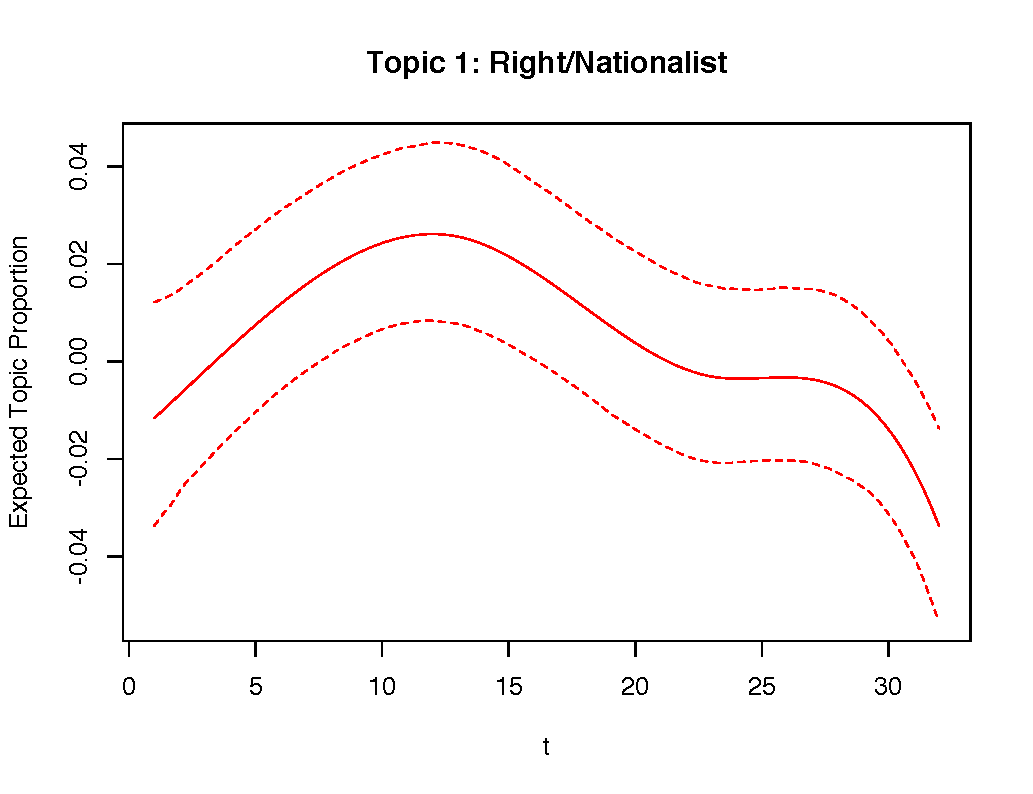
\includegraphics[width=\linewidth]{../../plots/presentation/estEffect_topic1.pdf}
  \end{subfigure}
  \begin{subfigure}[b]{0.4\linewidth}
    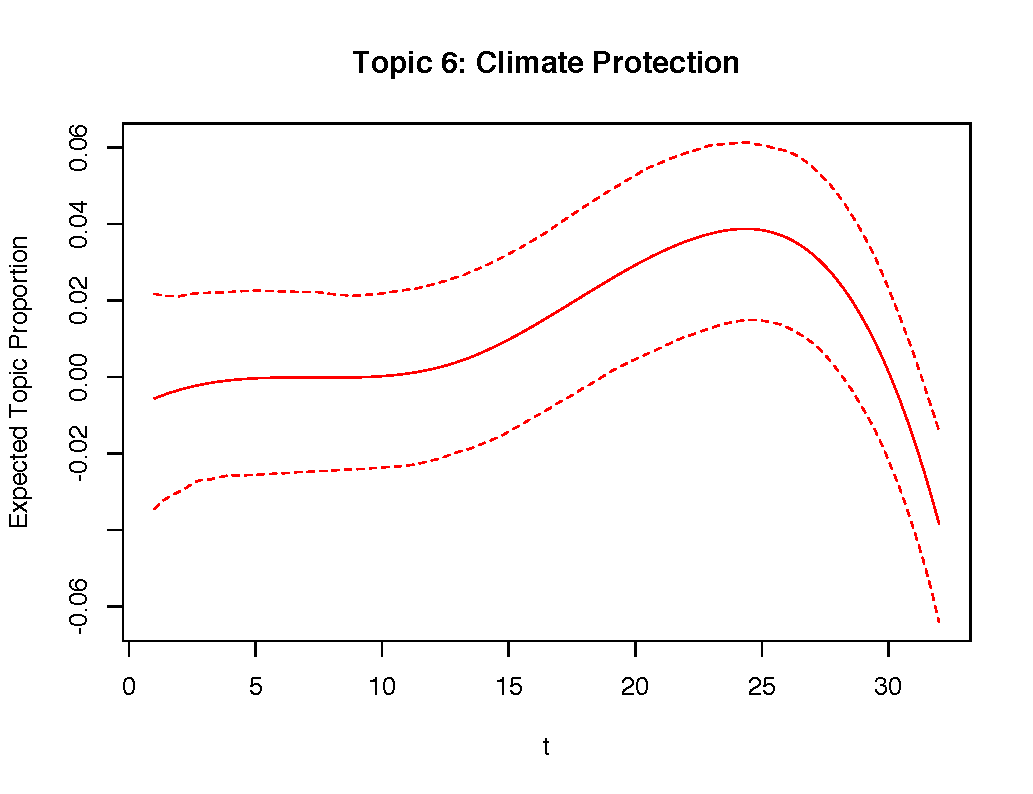
\includegraphics[width=\linewidth]{../../plots/presentation/estEffect_topic6.pdf}
  \end{subfigure}
  \caption{Emprical mean and 95\% credible intervals for topics 1 and 6 over time, estimated using \textit{estimateEffect} from the \textit{stm} package.}
  \label{fig:estEffect_topic16}
\end{figure}
\end{frame}

\begin{frame}
\frametitle{Covariate-level Topic Analysis}
\framesubtitle{Method of Composition: Extension of existing approach}
\begin{itemize}
\item Instead of OLS regression, we can use a beta regression or a quasibinomial GLM (both with logit-link) to adequately model proportions
\end{itemize}
\begin{figure}[h!]
  \centering
  \captionsetup{justification=centering,margin=2cm}
  \begin{subfigure}[b]{0.4\linewidth}
    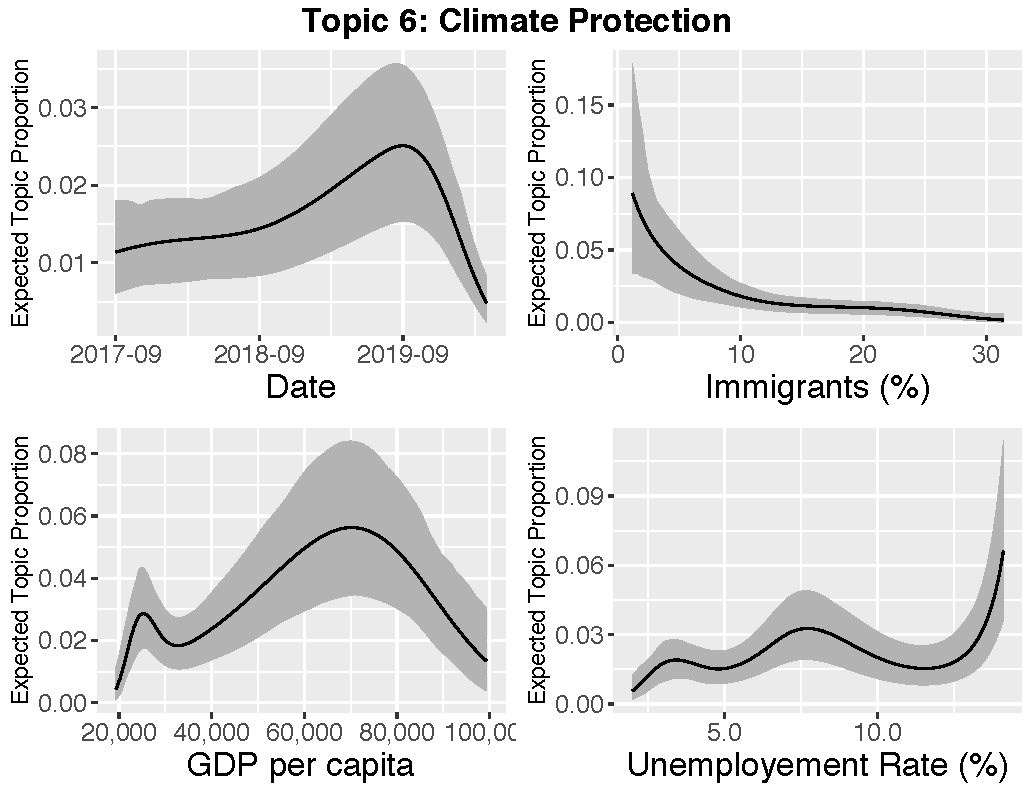
\includegraphics[width=\linewidth]{../../plots/presentation/quasi_t6_cont.pdf}
  \end{subfigure}
  \begin{subfigure}[b]{0.4\linewidth}
    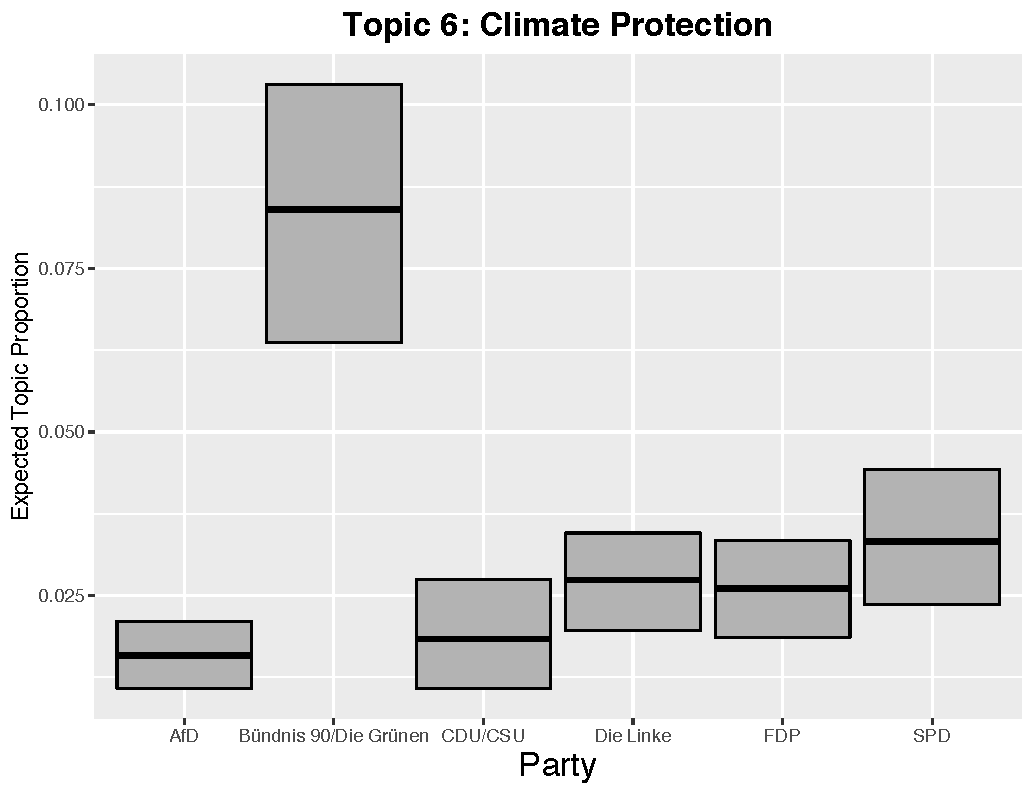
\includegraphics[width=\linewidth]{../../plots/presentation/quasi_t6_cat.pdf}
  \end{subfigure}
  \caption{Empirical mean and 95\% credible intervals, obtained using a quasibinomial GLM.}
  \label{fig:quasi_t46_cont}
\end{figure}
\end{frame}

\begin{frame}
\frametitle{Covariate-level Topic Analysis}
\framesubtitle{Mixing of Bayesian and Frequentist Approach}
\begin{itemize}
\item Regression within of method of composition is \textit{frequentist} regression
\item However, in STM $\tilde{\boldsymbol{\xi}}^*$ considered samples from (marginal, i.e., integrated over latent topic proportions) posterior of regression coefficients; only true by assuming uniform priors for $\boldsymbol{\xi}$
\item Caution: uncertainty from previous plots with respect to prediction of mean $\Rightarrow$ does \textit{not} reflect variation of topic proportions in data!
\item Better idea: fully Bayesian approach with more realistic priors and sampling from posterior predictive distribution to reflect variation of data
\end{itemize}
\end{frame}

\begin{frame}
\frametitle{Covariate-level Topic Analysis}
\framesubtitle{Fully Bayesian Approach: Idea}
\begin{itemize}
\item Idea: \textit{explicitly} perform Bayesian regression in second step of each iteration of method of composition
\item Modeling via beta regression (with normal priors centered around zero) in order to model proportions in $(0,1)$
\item Visualization: Sample proportions from posterior predictive distribution at end of each step of method of composition (i.e., conditioning on previously sampled $\boldsymbol{\theta}_{(k)}^*$) with covariate values $\boldsymbol{x}_{\text{pred}}$
\end{itemize}
\end{frame}

\begin{frame}
\frametitle{Covariate-level Topic Analysis}
\begin{itemize}
\item Predicted (empirical) mean mostly in line with results from previous analysis
\item Uncertainty now w.r.t.\ variation of topic proportions in data
\item Observed variation for topic proportions corresponds well to variation according to predictive posterior
\end{itemize}
\framesubtitle{Fully Bayesian Approach: Results}
\begin{figure}[h!]
  \centering
  \captionsetup{justification=centering}
  \begin{subfigure}[b]{0.4\linewidth}
    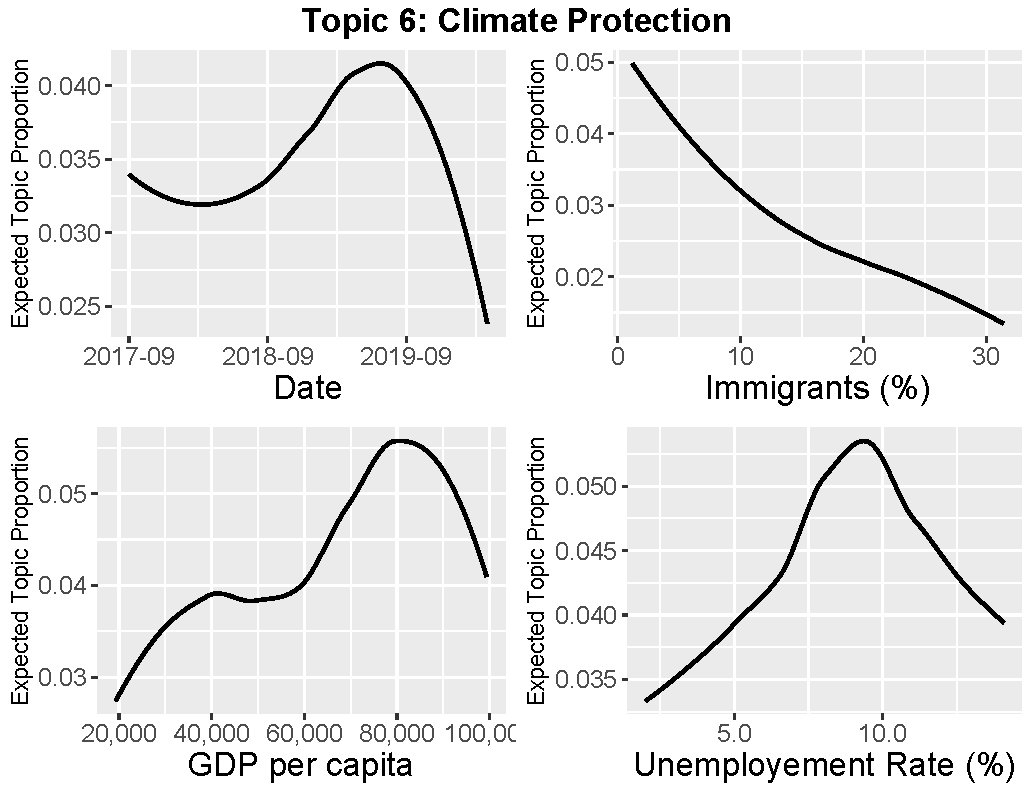
\includegraphics[width=\linewidth]{../../plots/presentation/stanbeta_t6_without_credible.pdf}
  \end{subfigure}
  \begin{subfigure}[b]{0.4\linewidth}
    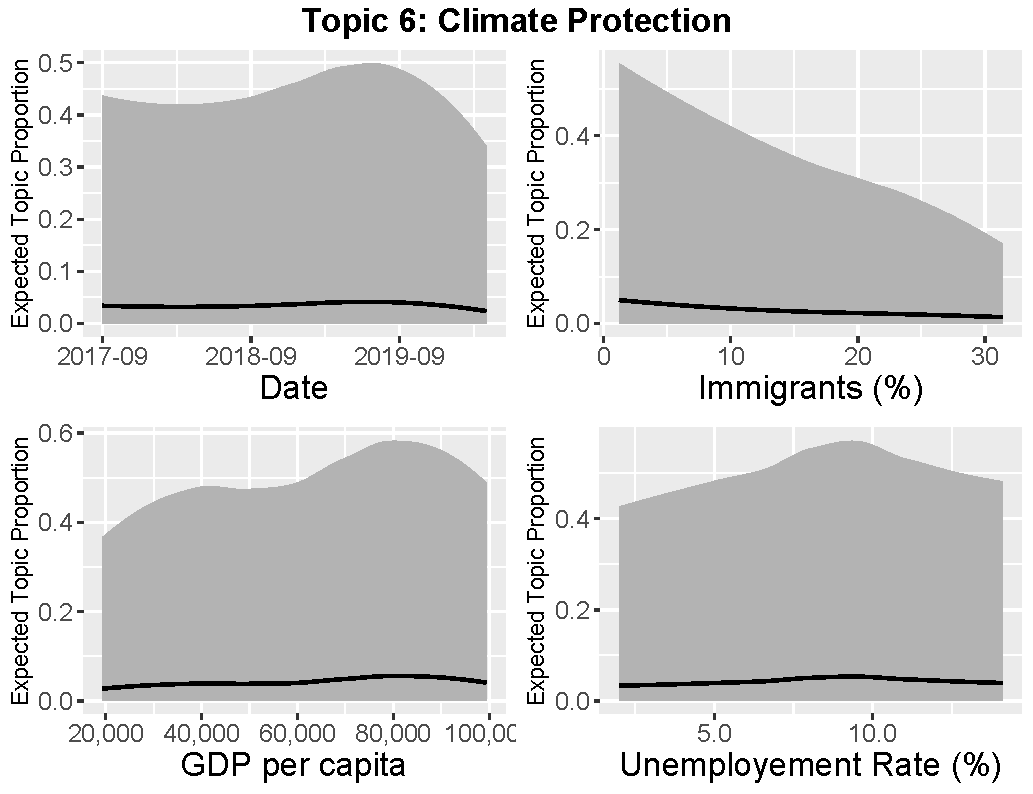
\includegraphics[width=\linewidth]{../../plots/presentation/stanbeta_t6_with_credible.pdf}
  \end{subfigure}
  \caption{Smooth effects without credible intervals (left) and smooth effects with 95\% credible intervals (right)}
  \label{fig:directassessment}
\end{figure}
\end{frame}

\begin{frame}
\frametitle{Covariate-level Topic Analysis}
\framesubtitle{Multivariate Modeling of Proportions}
\begin{itemize}
\item Remember, by assumption: $\boldsymbol{\theta}_d \sim \text{LogisticNormal}(\boldsymbol{\Gamma}^T\boldsymbol{x}_d^T, \boldsymbol{\Sigma})$
\item Logistic normal distribution assumes high dependence among individual components $\Rightarrow$ not fully taken into account in univariate modeling via, e.g., the beta distribution
\item Inference within STM involves finding estimates $\hat{\boldsymbol{\Gamma}}$ and $\hat{\boldsymbol{\Sigma}}$ $\Rightarrow$ Idea: plug estimates into logistic normal distribution
\item For given covariate value $\boldsymbol{x}_{\text{pred}}$, obtain topic proportion as $\boldsymbol{\theta}^*_d \sim \text{LogisticNormal}(\hat{\boldsymbol{\Gamma}}^T\boldsymbol{x}_{\text{pred}}^T, \hat{\boldsymbol{\Sigma}})$
\end{itemize}
\end{frame}

\begin{frame}
\frametitle{Covariate-level Topic Analysis}
\framesubtitle{Multivariate Modeling of Proportions}
\begin{itemize}
\item Plugging in $\boldsymbol{\Gamma}$ and $\hat{\boldsymbol{\Sigma}}$ is "na{\"i}ve" method: ideally sample prevalence parameters from their posterior $\Rightarrow$ would yield higher variation
\item However, not easily possible $\Rightarrow$ should be addressed in future implementations
\end{itemize}
\begin{figure}[h!]
  \centering
  \captionsetup{justification=centering}
  \begin{subfigure}[b]{0.4\linewidth}
    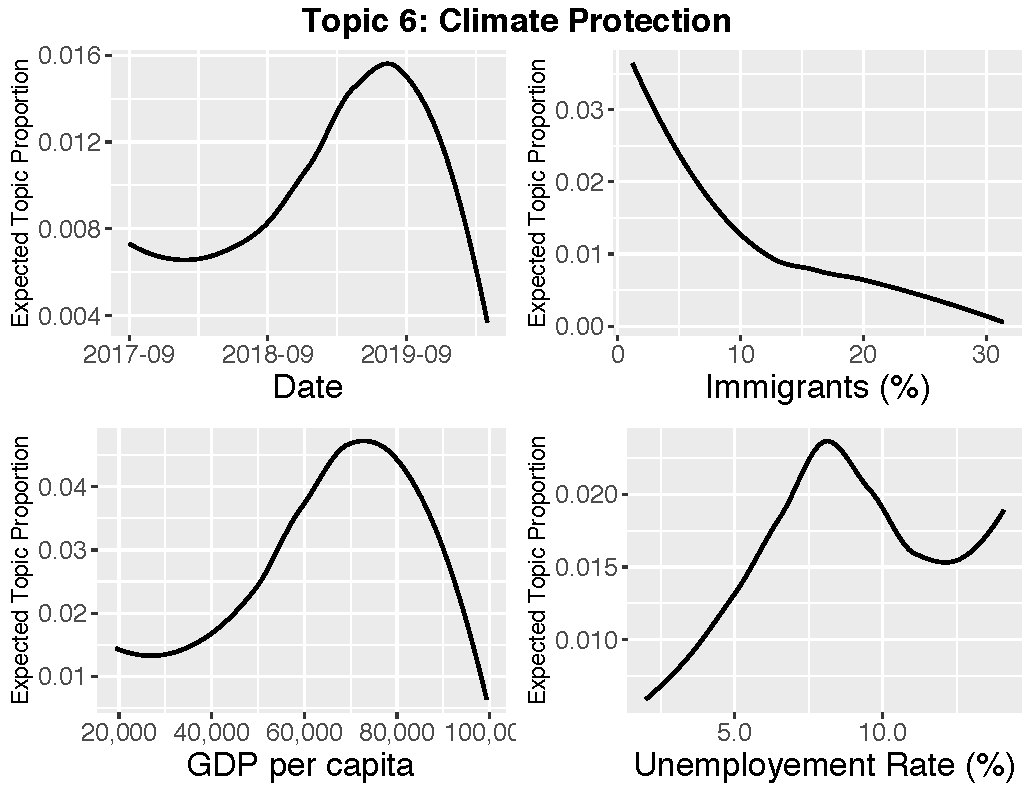
\includegraphics[width=\linewidth]{../../plots/presentation/direct_t6_without_credible.pdf}
  \end{subfigure}
  \begin{subfigure}[b]{0.4\linewidth}
    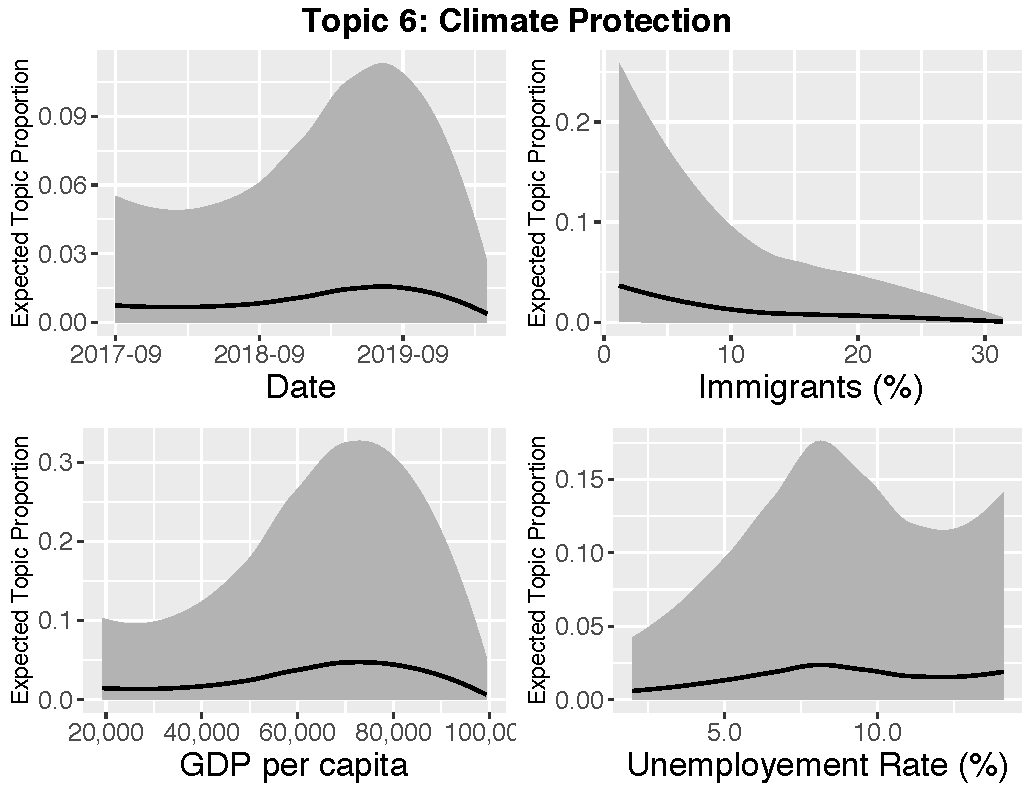
\includegraphics[width=\linewidth]{../../plots/presentation/direct_t6_with_credible.pdf}
  \end{subfigure}
  \caption{Smooth effects without credible intervals (left) and smooth effects with credible intervals (right)}
  \label{fig:directassessment}
\end{figure}
\end{frame}

\begin{frame}
\frametitle{Bibliography}
\printbibliography
\end{frame}
\end{document}